\documentclass[12pt]{article}
\usepackage{latexsym}
\usepackage{amssymb,amsmath}
\usepackage[pdftex]{graphicx}
\usepackage{epstopdf}


\topmargin = 0.1in \textwidth=5.7in \textheight=8.6in

\oddsidemargin = 0.2in \evensidemargin = 0.2in


\begin{document}

\begin{center}
COMPUTER SCIENCE 20, SPRING 2014 \\
Homework Problems\\
Invariants, Digraphs, and Relations\\
Author: Tawheed Abdul-Raheem
\end{center}

\smallskip

\begin{enumerate}
\item A directed graph $G$ has an \textit{Euler Tour} iff there is a closed walk in $G$ that uses every edge exactly once. 
\begin{enumerate}
\item List the sequence of nodes of one possible Euler Tour for the following graph: \\
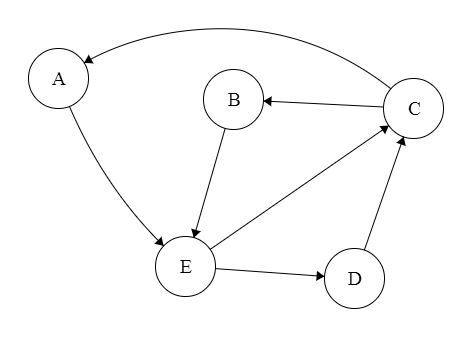
\includegraphics{eulertour}
\textbf{Solution: } An \textit{Euler Tour} is a path that uses every edge of a graph exactly once. The sequence of nodes for one possible \textit{Euler Tour} is: \\
$
\langle C \rightarrow A \rightarrow E \rightarrow C \rightarrow B \rightarrow E  \rightarrow D \rightarrow C\rangle
$
\item Show that in general, if a graph has an Euler Tour, then the in-degree of every vertex equals its out-degree.\\\\
    \textbf{\textit{Proof: }} Lets say that a simple cycle is one where there is exactly one visit to each vertex and a complex cycle is one that can have more than one visit to a vertex. By definition we know from a simple cycle that the number of in-degree is the same as the number of out-degree which in this case happens to be $1$. We further know that a complex cycle can be represented by multiple simple cycles. This imples that any vertex in an \textit{Euler Tour} has an equal number of in-degree as well as out-degree because of their representation. We can conclude that  if a graph has an Euler Tour, then the in-degree of every vertex equals its out-degree.

\end{enumerate}

\item A group of vertices $A$ in a graph is \textit{completely connected} if every pair of vertices in $A$ has a directed edge in both directions, and every vertex into $A$ has a self-loop. A \textit{partition} of a nonempty set $S$ is a way of dividing it into disjoint sets such that every element in $S$ is in exactly one of these subsets.
\begin{enumerate}
\item Show that a group of vertices in an equivalence class must be completely connected. \\\\
    \textbf{\textit{Proof:}} By definition, we know that inorder for an equivalence relation to exist, a given graph $G$, must be reflexive $(\forall x)(xRx)$, symmetric $(\forall xy) (xRy) \rightarrow (yRx)$ and transitive $(\forall xyz) (xRy \text{ AND } yRz \rightarrow xRz)$. Based on on the definition that we have established, we can attempt to prove by contradiction that an equivalence class must be completely connected, if a graph were to not have a reflexive property one can make the case that the graph is not completely connected. From this we can say that an equivalence class must be completely connected. 
\item  Prove that if $R$ is an equivalence relation on $S$, then the equivalence classes of $R$ constitute a partition of $S$ (show that every element of $S$ is in exactly one equivalence class of $R$).\\\\
    \textbf{\textit{Proof:}} For a given set $S$ lets assume that $R$ is an equivalence relation on a given set. Let the equivalence class of $a \implies \{ b| aRb, b \in S \}$ The given graph looks something like the below image.

    \begin{center}
    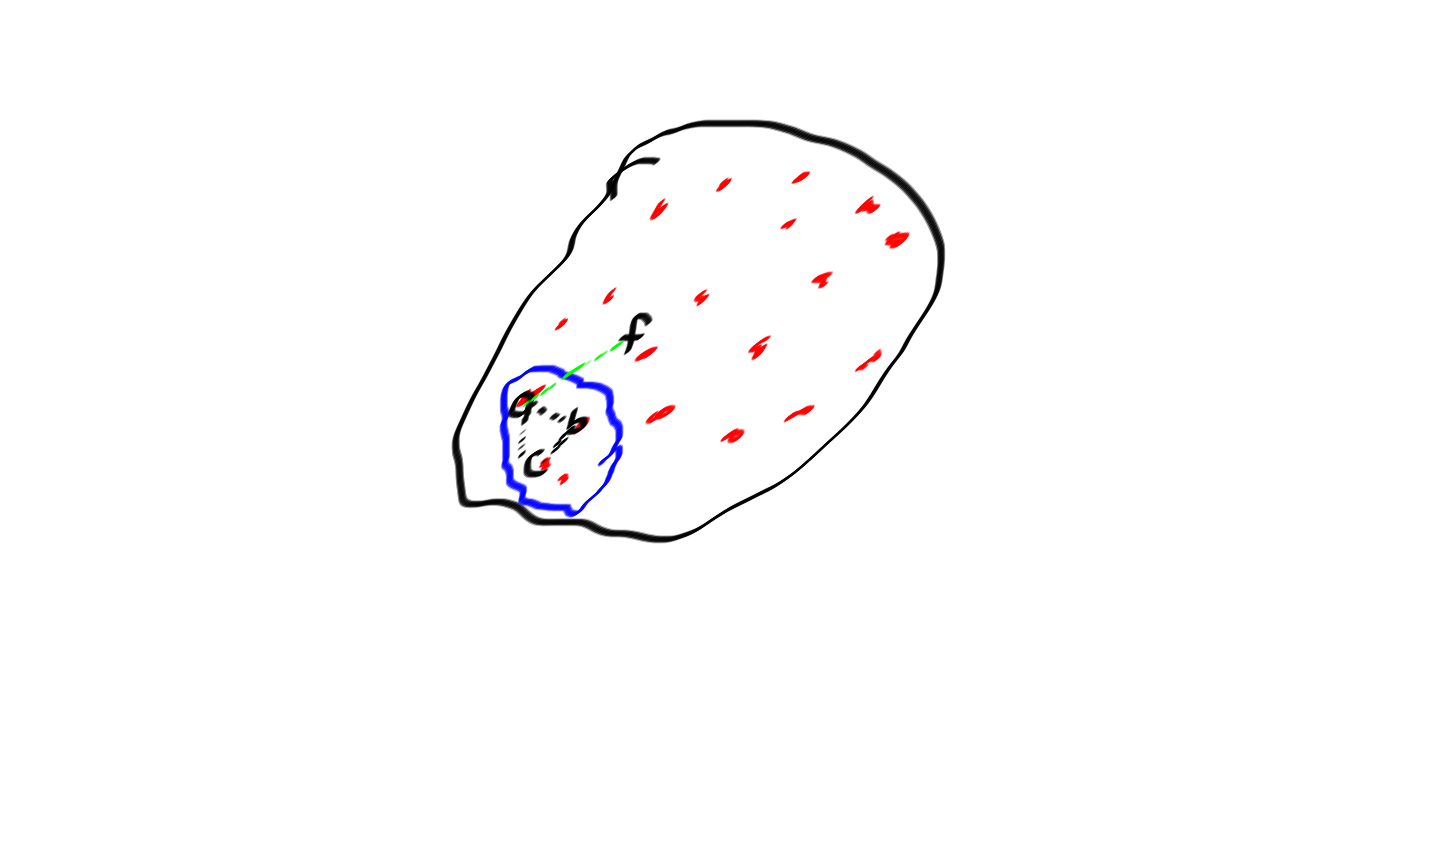
\includegraphics[scale=0.24]{num2.png}
    \end{center}
    \begin{itemize}
            \item From the above set we can establish the claim that everything in the little set ($Subset$)  is related to one another based on our definition of an equivalence relation - reflexive, symmetric and transitive.
                \item We can also establish the claim that nothing in the $subset$ is related to anything outside of that subset. We can proof this by contradiction, lets say that the element $b$ is related to the element $f$. By definition (the equivalence of an element in a given subset is the same as the equivalence class of everything) this will mean that all the items in the $subset$ is also related to the $f$ which is flase. This implies that we cannot have anything in our subset relate to anything outside of the set. This tight coupling of the elements of the subset forms a partition in our big set. 
    \end{itemize}
    From what we have derive from the above argument, we can take the big set and look at each of the element's equivalence class  and then apply the above to form a pair-wise disjoint (partition)
    \end{enumerate}

\item Recall that a binary relation $R \subseteq A \times A$ is the set of pairs of elements in $A$ that satisfy the relation. Let $R_1$ and $R_2$ be arbitrary equivalence relations on a set $A$. For each of the following, determine whether it must also be an equivalence relation. If so, prove it. If not, give a counterexample.
\begin{enumerate}
\item $R_1 \cup R_2$ - Non equivalence and below is the counter example
    \begin{center}
    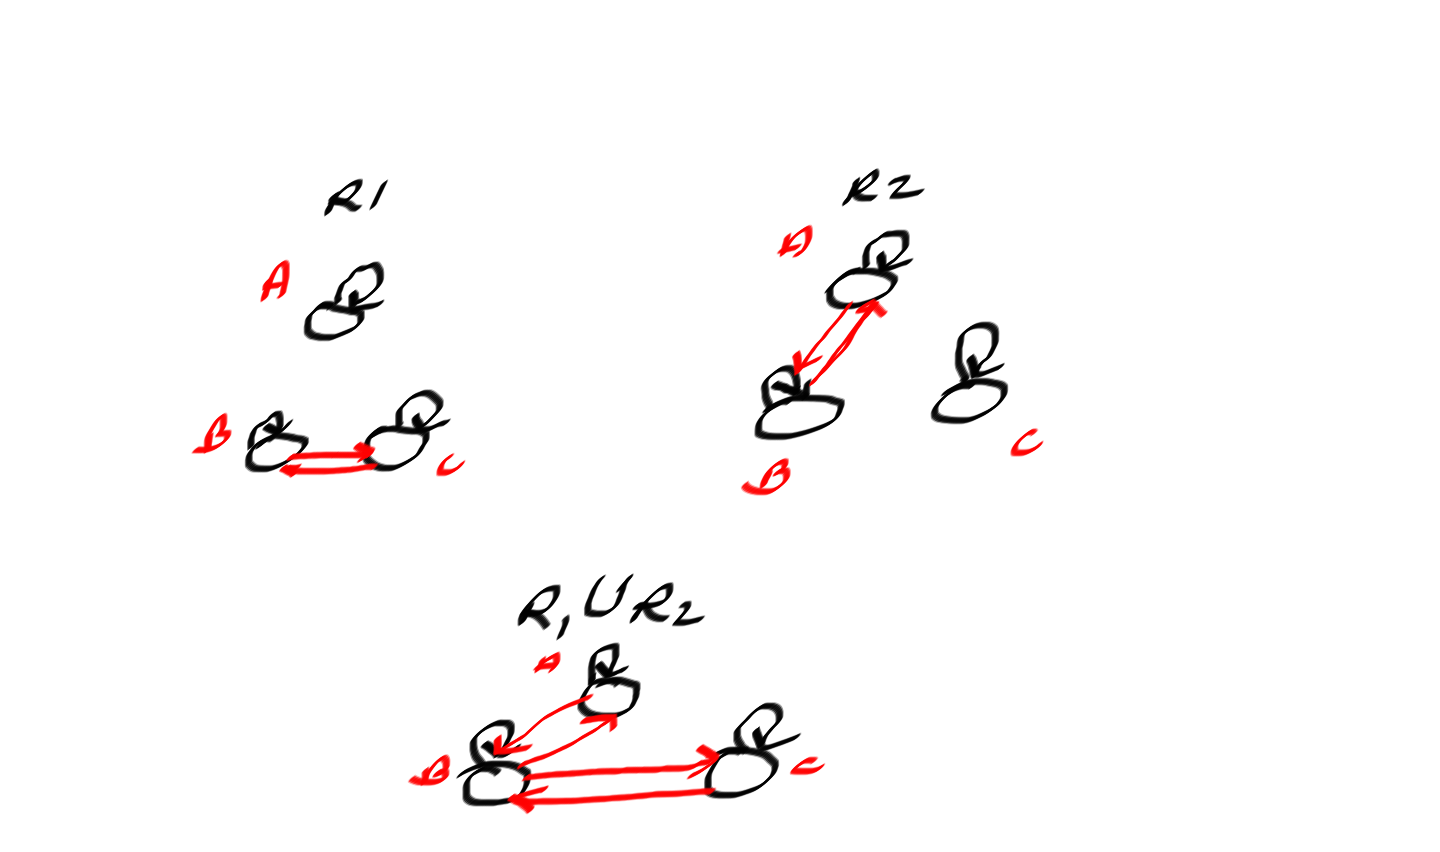
\includegraphics[scale=0.24]{3a.png}
    \end{center}
\item $R_1 \cap R_2$ - This is an equivalence relation  and thus we will prove it for all the properties of an equivalence relation\\
    \textbf{\textit{Proof: }} \\
    First, since $R_1$ and $R_2$ are both reflexive, this means that for every element a of $S$, $(a,a) \in R_1$ and $(a,2) \in R_2$. Which implies that for every element $a$ of $S$, $(a,a) \in R_1 \cap R_2$ so the relation is reflexive\\
    Based on our definition of symmetry, we calim that $R_{1}$ and $R_2$ are symmetric and that some $(a,b) \in (R_{1} \in R_2)$ From this we can also prove that $(b,a) \in (R_{1} \cap R_2)$ Since $(a,b) \in (R_{1} \cap R_2)$ both $(a,b) \in R_{1}$ and $(a,b) \in R_2$. Since both $R_{1}$ and $R_2$ are symmetric then it follows that $(b,a) \in R_{1} \text{ and } (b,a) \in R_2$ \\
    Transitivity of $R_1 \cap R_2$ is equivalent to the implication that if $(a, b) \in$ 
    $(R_1 \cap R_2) \text{ and }  (b, c) \in (R_1 \cap R_2), t\text{ then } (a, c) \in (R_1 \cap R_2)$. Because we are dealing with the intersection of the two sets which basically mean that whatever in $R_1 \textbf{ must } \text{ also be presesnt in } R_2$

\item $R_1 \setminus R_2$ - Non equivalence and below is the counter example
    \begin{center}
    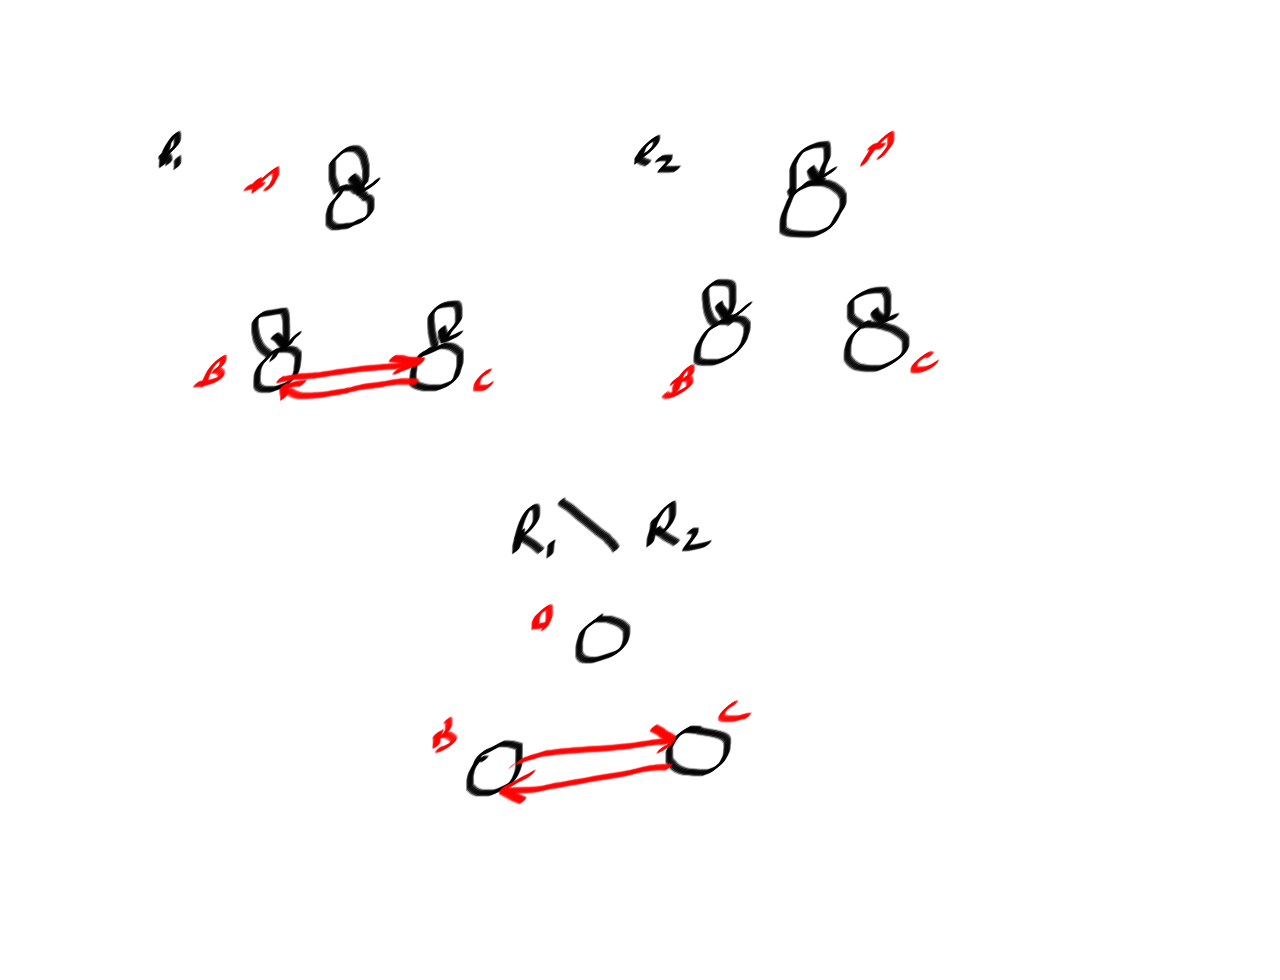
\includegraphics[scale=0.24]{3c.png}
    \end{center}
\end{enumerate}

\item Consider a regular unshuffled deck of cards, arranged from top to bottom as follows:
\[A\heartsuit 2\heartsuit...K\heartsuit A\spadesuit 2\spadesuit...K\spadesuit A\clubsuit 2\clubsuit ... K\clubsuit A\diamondsuit 2\diamondsuit...K\diamondsuit\]
We only allow two operations on the deck: \textit{inshuffling} and \textit{outshuffling}. In both, the shuffle is done by cutting the deck exactly in half, and taking the top half into your right hand and the bottom half in your left hand. Then shuffle them together by perfectly interlacing the cards; that is, the shuffled deck will consist of one card from the left, one from the right, one from the left, one from the right, etc. The top card of the shuffled deck comes from the right hand in an outshuffle and from the left hand in an inshuffle.

Use the Invariant Principle to prove that you cannot make the entire first half of the deck black through a sequence of inshuffles and outshuffles. (Try doing a couple shuffles and looking for a trend, and then prove that this property is invariant). \\

\textbf{\textit{Proof: }} Using the Invariant principle to prove that you cannot make the entire half of the deck black through a sequence on inshuffles and outshuffles\\
\begin{center}
    $P(n) := $ No matter how many shuffles that occur the two halfves are always going to be symmetric of one another.
\end{center}
\textbf{ Base Case. (0 shuffles) } If we take the original deck of cards as the way it is, we can observe that each half is symmetric of the other.\\
\textbf{Inductive step: } Assuming that $P(n)$ is true, we need to show that this is also true for any $(n+1)$ in and outshuffles. For every step that happens we see a convergence from the middle and observe a symmetry, each step involves a step backwards from the previous step. After $52$ of such shuffles we can see that the card gets back to it original position. Because we are dealing with two halfves of different in no point would be have all colors one side because of their symmetric nature.
\end{enumerate}
\end{document}
